% Text which is good, but should be placed elsewhere in another work.
We seek in this work to describe the influence PMFs had on the dense electron-positron $(e^{+}e^{-})$ plasma epoch in the temperature range $2\MeV>T>0.02\MeV$ in the early universe. There are three conventional explanations~\cite{batista2021gammaray} for the existence of IGMF:
\begin{itemize}
    \item [1.] \textbf{Primordial fields} - Cosmic primordial magnetic fields (PMF) are produced in the universe before the recombination epoch possibly as far back as inflation. Such fields would arise from the cosmic-scale polarization of the early universe, phase transitions, or magnetogenesis from the breakdown of some unknown field.
    \item [2.] \textbf{Dynamo amplification} - Initially small \lq\lq seed\rq\rq\ magnetic fields dynamically reorganize charged matter fluids amplifying the total magnetic flux in a process called dynamo. Such seed fields may be primordial or astrophysical in origin.
    \item [3.] \textbf{Astrophysical sources} - Late times development of IGMF arises from stars, supernova and active galaxy nuclei (AGN) producing galactic outflows of charged matter which would contaminate and magnetize regions between galaxies.
\end{itemize}
Even if IGMFs are found to be produced by some mixture all three scenarios listed above, the existence of PMFs would be uniquely interesting because of their effects on (or generation within) the early universe primordial plasmas which populated the universe before recombination.

Other candidates include: inflationary magnetogenesis~\cite{subramanian2009magnetic}, electroweak transition~\cite{vachaspati2020progress}, QGP-hadronization eras~\cite{bali2011qcd}. It was found in~\cite{gopal2004generation} that the electron, proton, photon plasma of the immediate pre-recombination era generates (from density fluctuations) a tiny contemporary field of ${\cal B}\simeq10^{-30}{\rm\ G}$ far below the known IGMF bound or necessarily seed field size for dynamo.

Within a homogeneous field regime, the magnetic field varies over cosmic expansion as
\begin{align}
    \label{cosmicscale}
    {\cal B}(t)={\cal B}_{0}\left(\frac{a(t_0)}{a(t)}\right)^{\kappa}\rightarrow{\cal B}(z)={\cal B}_{0}\left(1+z\right)^{\kappa}\,,
\end{align}
where $a(t)$ is the scale factor for the universe's expansion (as given by the FLRW metric), $z$ is the redshift, and ${\cal B}_{0}$ is the comoving value of the magnetic field defined by the contemporary value of the magnetic field today. The parameter $\kappa$ is then determined by the physical origin of the magnetic field. For scale-invariant PMFs, $\kappa=2$ as to conserve the total magnetic flux through comoving surfaces~\cite{durrer2013cosmological}. Magnetic fields which are generated through other mechanisms~\cite{pomakov2022redshift} (such as dynamo or astrophysical sources) will have values which differ and in general $\kappa\rightarrow\kappa(z)$ can be parameterized as a function of redshift. Even for PMFs, the measured value of $\kappa$ will deviate to account for the change in flux from large scale structure formation in the mid to late universe's evolution.

Field strengths of around a tenth of a nanoGauss is also near the more stringent upper bound for PMFs found in~\cite{pshirkov2015new,jedamzik2019stringent}. Conversely, measurements of synchrotron radiation from \lq\lq blazar\rq\rq\ AGN whose jets are pointed towards the Earth provide the lower bound~\cite{neronov2010evidence,taylor2011extragalactic} on IGMFs seen in \req{igmf}. Due to cosmological redshift, and the conservation of magnetic flux through a comoving surface, PMFs would have extraordinary field strengths during the various primordial plasmas of the early universe subject to whatever temperature they were initially generated in.

{\xblue We point again to the} electron-positron number density ratio relative to the baryon number density (shown in~\rf{fig:densityratio}) in the temperature range $2000\keV>T>20\keV$ as a consequence for the $e^{+}e^{-}$ results we have shown in.

%%%%%%%%%%%%%%%%%%%%%%%%%%%%%%%%%%%%%%%
\begin{figure}[ht]
    \centering
    \begin{subfigure}[b]{0.49\textwidth}
        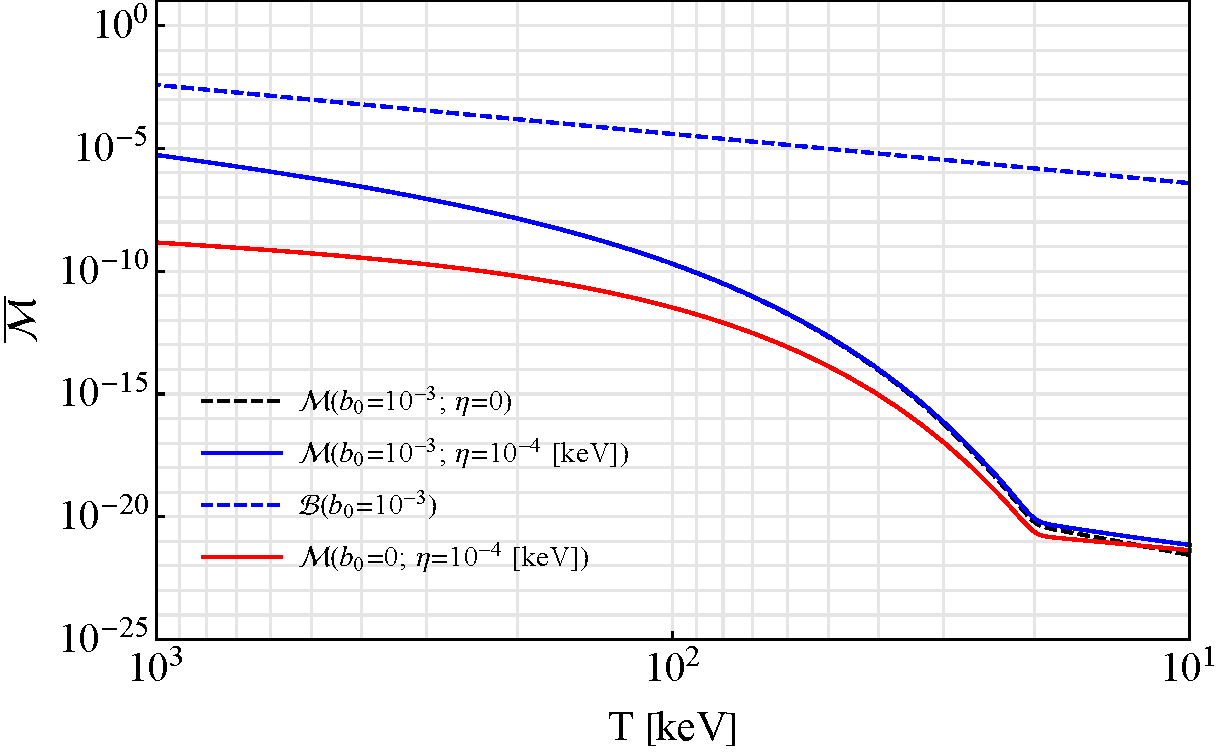
\includegraphics[width=\textwidth]{SpinLowFugacity.pdf}
    \end{subfigure}
    \hfill
    \begin{subfigure}[b]{0.49\textwidth}
        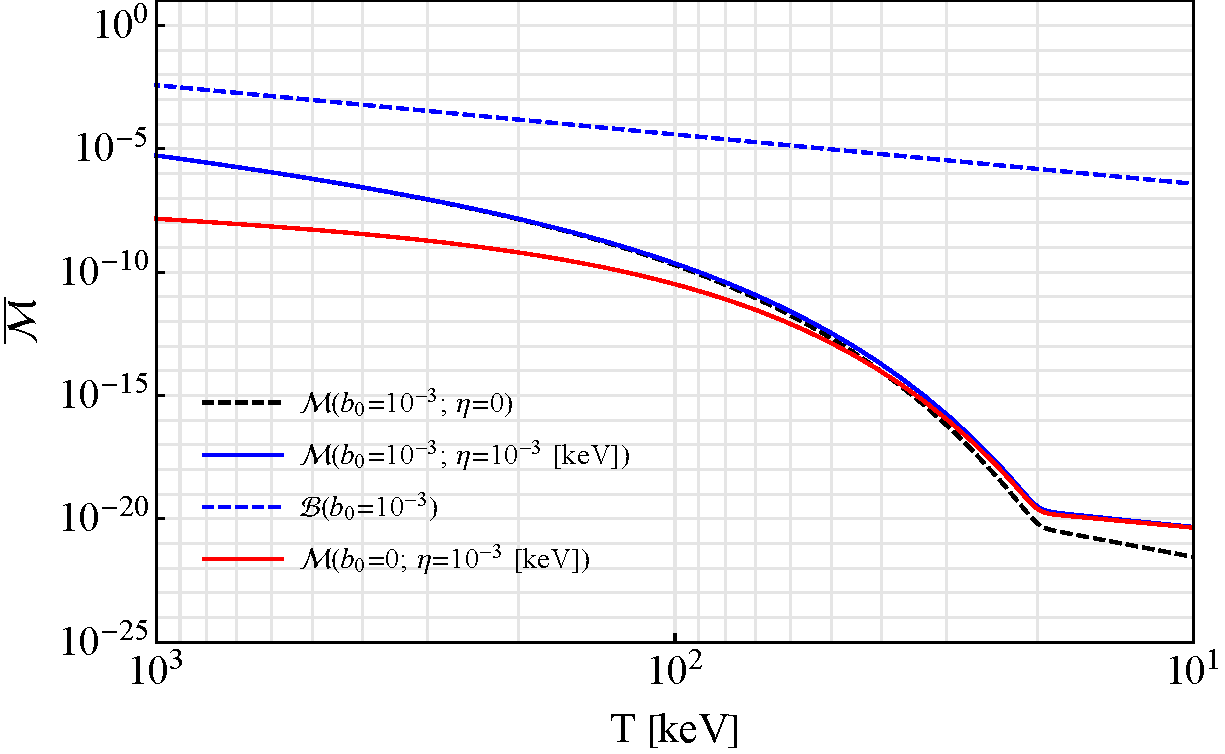
\includegraphics[width=\textwidth]{SpinMidFugacity.pdf}
    \end{subfigure}
    \caption{to be written}
    \label{fig:spin}
\end{figure}
%%%%%%%%%%%%%%%%%%%%%%%%%%%%%%%%%%%%%%%